\documentclass[12pt, a4paper]{article}

\usepackage[nottoc,notlot,notlof]{tocbibind}
\usepackage[pdftex]{graphicx}
\usepackage[pdftex,hypertexnames=false]{hyperref}
\hypersetup{colorlinks=true,
  unicode=true,
  linkcolor=black,
  citecolor=black,
  urlcolor=black,
  bookmarksopen=true}
\usepackage[numbers,sort&compress]{natbib}
\usepackage{svg}
\usepackage{textcomp}
\usepackage{amsmath}
\usepackage{listings,xcolor}
\usepackage{mathtools}
\usepackage[final]{pdfpages}
\usepackage{verbatim}
\usepackage{fancyhdr}

\title{\textbf{Dokumentace semestrální práce} \\KIV/IR}
\author{Vojtěch Danišík}
\begin{document}

\begin{titlepage} 
	\newcommand{\HRule}{\rule{\linewidth}{0.5mm}} 
	\begin{center}
	
\includegraphics[width=12cm]{img/fav_logo}\\
	\end{center}
	\textsc{\LARGE Západočeská univerzita v Plzni}\\[1.5cm] 	
	\textsc{\Large Vyhledávání informací}\\[0.5cm] 
	\textsc{\large KIV/IR}\\[0.5cm] 
	\HRule\\[0.4cm]
	{\huge\bfseries Dokumentace semestrální práce}\\[0.4cm] 
	\HRule\\[1.5cm]

	\begin{minipage}{0.4\textwidth}
		\begin{flushleft}
			\large
			Vojtěch \textsc{Danišík}\newline
			A19N0028P\newline
			danisik@students.zcu.cz
		\end{flushleft}
	\end{minipage}
	\vfill\vfill\vfill
	\begin{flushright}
	{\large\today}
	\end{flushright}
	\vfill 
\end{titlepage}
\newpage
\tableofcontents
\newpage

\section{Zadání}
Implementace vlastního systému automatické indexace a vyhledávání dokumentů.
Minimální nutná funkčnost semestrání práce pro získání 15 bodů/zápočtu:
\begin{itemize}
\item Tokenizace
\item Preprocessing (stopwords remover, stemmer/lemmatizer)
\item Vytvoření in-memory invertovaného indexu
\item tf-idf model, cosine similarity, vyhledávání pomocí dotazu vrací top X výsledků seřazených dle relevance
\item Vyhledávání s pomocí logických operátorů AND, OR, NOT, podpora závorek pro vynucení priority operátorů
\item Možnost zaindexování poskytnutých dat a dat stažených na cvičení (1. cvičení Crawler)
\end{itemize}
Nadstandardní funkčnost (lze získat až dalších 15 bodů):
\begin{itemize}
\item File-based index (1b),
\item Pozdější doindexování dat (1-2b) - přidání nových dat do existujícího indexu.
\item Ošetření např. HTML tagů (1b),
\item Detekce jazyka dotazu a indexovaných dokumentů (1b),
\item Vylepšení vyhledávání (1-?b),
\item Vyhledávání frází (i stop slova)(1b),
\item Vyhledávání v okolí slova (1b),
\item Více scoring modelů (1b),
\item Indexování webového obsahu (2-3b) - zadam web, program stahne data a rovnou je zaindexuje do existujícího indexu,
\item Další předzpracování normalizace (1b),
\item GUI/webové rozhraní (2b),
\item Napovídání keywords (1b),
\item Podpora více polí pro dokument (např. datum, od do)(1b),
\item CRUD indexovaných dokumentů (2b),
\item Zvýraznění hledaného textu v náhledu výsledků (1b),
\item Dokumentace psaná v TEXu (1b),
\item Implementace dalšího modelu (použití sémantických prostorů) (1-?b),
\item Atd. (xb)
\end{itemize}
\newpage

\section{Analýza}
\subsection{Invertovaný index}
Invertovaný index je datová struktura používaná pro fulltextové vyhledávání v rozsáhlých kolekcích dokumentů. Obvykle se jedná o seznam významných slov (nejsou součástí množiny stop slov), upravených pomocí stematizace (nalezení kmene slova) a lemmarizace (nalezení základního tvaru slova). Ke každému takovému slovu je přiřazen seznam dokumentů, ve kterých se slovo vyskytuje. Účelem invertovaného indexu je umožnit rychlé vyhledávání za cenu dodatečných operací v okamžiku přidání dokumentu do databáze. Příklad invertovaného indexu lze vidět na obrázku \ref{fig:index}.
\begin{figure}[h]
	\centering
	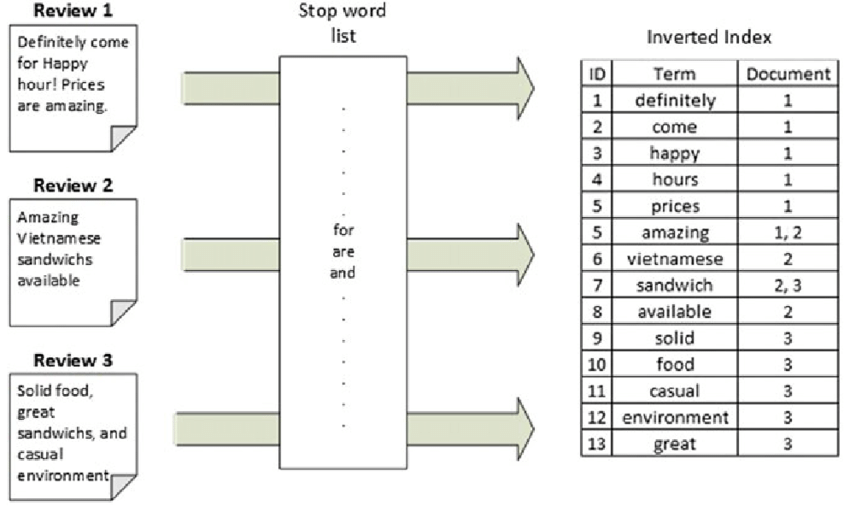
\includegraphics[width=14cm]{img/inverted_index.png}
	\caption{Hlavní okno}
	\label{fig:index}
\end{figure}
\newpage
\subsection{TF-IDF}
TF-IDF, neboli \textbf{T}erm \textbf{F}requency - \textbf{I}nverse \textbf{D}ocument \textbf{F}requency, je numerické číslo, které reprezentuje důležitost slova pro daný dokument v kolekci nebo v korpusu. Při výpočtu hodnoty TF-IDF se používají 2 hodnoty:
\begin{itemize}
\item {TF} - Term Frequency- četnost slova v dokumentu.
\item {IDF} - Inverse Document Frequency - Převrácená četnost slova ve všech dokumentech (vzoreček viz \ref{eq:idf}, kde \textit{N} je počet všech dokumentů v korpusu, \textit{d} je specifický dokument v seznamu dokumentů \textit{D} a \textit{t} je dané slovo v dokumentu \textit{d}).
\begin{equation}
idf(\textit{t},\textit{D}) = log\textsubscript{10} \frac{N}{| d \in D : t \in d |}
\label{eq:idf} 
\end{equation}
\end{itemize}

Výslednou hodnotu TF-IDF lze vypočítat pomocí vzorečku \ref{eq:tfidf}.
\begin{equation}
tfidf(t,d,D) = log\textsubscript{10}(1 + tf(t,d)) \cdot idf(t,D)
\label{eq:tfidf} 
\end{equation}

TF-IDF je v dnešní době nejčastěji používaná hodnotící metodika u webových vyhledávačů (Google, Seznam , ...) pro zadaný textový řetězec. Pro výpočet TF-IDF hodnot lze použít více variant (více sofistikované metody jsou pouze upravené varianty základního modelu).


\subsection{Vector Space Model}
Vector Space Model je algebraický model, který reprezentuje objekty (např. textové dokumenty) jako vektory reálných hodnot (např. TF-IDF hodnoty). Využívá se hlavně pro filtraci / získávání informací. indexaci a zjišťování relevance objektů.

Ve VSM jsou všechny objekty reprezentovány jako objekty, kdy každá dimenze vektoru odpovídá jednomu slovu. Pokud se dané slovo vyskytuje v dokumentu, je příslušná dimenze nenulová. Příklad vektoru dokumentu viz příklad \ref{eq:vector}.
\begin{equation}
\begin{aligned}
d\textsubscript{j} = (w\textsubscript{1,j}, w\textsubscript{2,j}, ..., w\textsubscript{t,j}) \\
q = (w\textsubscript{1,q}, w\textsubscript{2,q}, ..., w\textsubscript{n,q})
\end{aligned}
\label{eq:vector} 
\end{equation}
Pro zjištění přesnosti mezi dvěma dokumenty se používá Kosinova podobnost (Cosine similarity). Kosinova podobnost je metoda pro zjištění hodnoty podobnosti mezi dvěma nenulovými vektory v unitárním prostoru. Vzoreček pro výpočet kosinovy podobnosti viz vzorec \ref{eq:cosine}.
\begin{equation}
\begin{aligned}
cos(d\textsubscript{j}, q) = \frac{d\textsubscript{j} \cdot q}{|| d\textsubscript{j} ||  || q ||} = \frac{\sum_{i=1}^N w\textsubscript{i,j}w\textsubscript{i,q}}{\sqrt{\sum_{i=1}^N w^2\textsubscript{i,j}} \sqrt{\sum_{i=1}^N w^2\textsubscript{i,q}}}
\end{aligned}
\label{eq:cosine} 
\end{equation}

\newpage

\section{Implementace}
\subsection{Indexace}
\subsubsection{Preprocessing}
V aplikaci byli použity 2 typy dokumentů:
\begin{itemize}
\item \textbf{Školní} - Jako data použitá pro preprocessing byly použity - titulek a text dokumentu.
\item \textbf{Crawlered} - Jako data použitá pro preprocessing byly použity všechny položky dokumentu.
\end{itemize}
Preprocessing se skládá z několika kroků:
\begin{enumerate}
\item \textbf{Převedení velkých znaků na malé znaky}
\item \textbf{Tokenizace} - Při tokenizaci dat dokumentu se použije speciální regex, který data rozparsuje na jednotlivá slova (případně celé webové stránky). Pokud tato slova se nevyskytují v seznamu stopslov a nejsou jednoznaková, tak se přidají do seznamu slov.
\item \textbf{Stematizace} - Všechna slova která prošla tokenizací jsou následně ostemována. Jako použitý stemmer byl využit \textbf{CzechStemmerAggresive} od pana Ljiljana Dolamiče. Stemmer se snaží najít nejlepší možný kmen daného slova.
\item \textbf{Odstranění diakritiky} - Po stematizaci je ze slova odstraněna veškerá diakritika pomocí speciálního regexu. Po odstranění diakritiky je slovo uloženo do invertovaného indexu, který s ním dále pracuje.
\end{enumerate}
\subsubsection{Invertovaný index}
Invertovaný index je v aplikaci reprezentován speciální HashMapou, kde klíč je dané slovo a hodnota reprezentuje IDF hodnotu slova a seznam dokumentů obsahující dané slovo.

Každý dokument v sobě obsahuje vlastní slovník, kdy klíč je slovo z dokumentu a hodnota reprezentuje TF-IDF pro dané slovo v daném dokumentu. Zároveň v sobě obsahuje i unikátní indetifikátor na původní dokument a střední hodnotu (která se poté použije při počítání kosinovy podobnosti). Struktura celého invertovaného indexu lze vidět na obrázku \ref{fig:index}.

\begin{figure}[h]
	\centering
	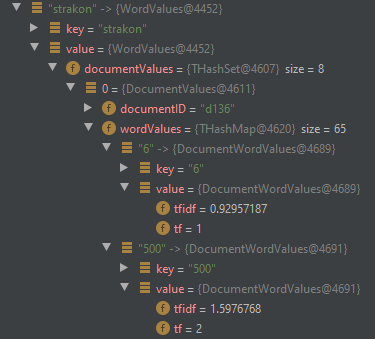
\includegraphics[width=10cm]{img/index.png}
	\caption{Struktura invertovaného indexu}
	\label{fig:index}
\end{figure}

Sestavování invertovaného indexu se skládá ze tří kroků:
\begin{enumerate}
\item \textbf{Vytvoření slovníku} - Vytváření slovníku probíhá při samotném preprocessingu, kdy se již upravené slovo ukládá jak do hlavního slovníku, tak i do slovníku aktuálně zpracovávaného dokumentu (objekt, který obsahuje hodnoty pro indexaci, ne přímo dokument). Zároveň se také uloží reference na tento dokument do seznamu dokumentů pro dané slovo.
\item \textbf{Výpočet IDF hodnot} - Po vytvoření slovníku se provede výpočet IDF hodnoty pro všechny slova v hlavním slovníku pomocí vzorečku \ref{eq:idf}.
\item \textbf{Výpočet TF-IDF hodnot} - Po vypočítání IDF hodnot pro slova ve slovníku se provede výpočet TF-IDF hodnot pro všechny slova ve slovníku ve všech dokumentech podle vzorečku \ref{eq:tfidf}. Zároveň se vypočítává i střední hodnota pro daný dokument.
\end{enumerate}

\subsection{Vyhledávání}
Pro vyhledávání v dokumentech byly implementovány 2 vyhledávací modely - Vector Space Model a Boolean.
\subsubsection{VSM}
Pokud si uživatel navolí vyhledávání v dokumentech pomocí Vector Space Modelu, tak se nad zadanou query provede stejný proces jako v případě indexace dokumentů (tokenizace, stematizace, ...). Po zaindexování query se provede výpočet TF-IDF hodnot pro všechny slova v dané query. 

Samotné vyhledávání probíha porovnáváním kosinových podobností mezi jednotlivými dokumenty a zadanou query. Před samotným počítáním kosinovy podobnosti jsou vybrány ty dokumenty, který obsahují alespoň jedno slovo ze zadané query. Mezi těmito dokumenty a zadanou query jsou následně vypočítány kosinovy podobnosti (i se skalárním součinem, viz vzorec \ref{eq:cosine}). V aplikaci jsou následně zobrazeny pouze nejvíce relevantní dokumenty k zadané query (počet nejrelevantnějších dokumentů si uživatel vybírá sám).
\subsubsection{Boolean}
Pokud si uživatel zvolí Boolean vyhledávání, je očekávána validní query. Lze používat operátory \textbf{AND}, \textbf{OR} a \textbf{NOT}.

Pro parsování boolean query byla použita třída \textbf{PrecedenceQueryParser} z \textbf{Lucene} knihovny. Bohužel se zde naskytl jeden veliký problém - dotazy obsahující \textit{... AND NOT ...} nebo \textit{... OR NOT ...} byly špatně zpracovány. Proto ještě před samotným použitím parseru se daná query musela upravit tak, aby zadaný dotaz byl dobře zpracovatelný. To zahrnovalo obalení daného operátoru \textbf{NOT} společně s následující klauzulí do jednoduchých závorek. Po této úpravě již parser neměl sebemenší problém správně rozparsovat danou query.

Samotné vyhledávání probíhá následovně:
\begin{enumerate}
\item \textbf{Úprava dotazu} - Samotná úprava spočívá v obalení \textbf{NOT} operátoru a klauzule do jednoduchých závorek. Tato úprava funguje tak, že daný dotaz rozparsuje na jednotlivé znaky pomocí mezer. Následně se tyto tokeny kontrolují na prezenci tokenu \textbf{NOT}, a pokud se takový token najde. Pokud se za operátorem \textbf{NOT} nevyskytuje žádná závorka, je obalení do závorek jednoduché. Pokud se zde objevuje závorka, tudíž klauzule, tak je provedeno rekurzivní volání tatéž metody, která provede následující část query.
\item \textbf{Parsování dotazu} - Parsování se provede pomocí \textbf{PrecedenceQueryParser}, který daný dotaz rozparsuje (vynucuje prioritu přes závorky a upřednostňuje AND před OR).
\item \textbf{Zpracování dotazu} - Zpracování dotazu probíhá rekurzivně, kdy se daný dotaz rozparsuje na klauzule, které jsou následně dále zpracovávány. Pokud je klauzule pouze \textbf{Term}, tak se vrátí seznam dokumentů obsahující daný term. Pokud klauzule obsahuje podklauzule, je provedeno další rekurzivní volání pro všechny podklauzule. Po zpracování všech klauzulí probíhá vyhodnocování operátorů. Jeden výsledek je roven ID dokumentu.
	\begin{itemize}
	\item \textit{AND} - Nad výsledky dvou \textbf{Term}ů je proveden průnik hodnot (ID dokumentů).
	\item \textit{OR} - Výsledky dvou \textbf{Term}ů se sloučí.
	\item \textit{NOT} - Provede se negace výsledků - Ze všech zaindexovaných dokumentů se vyloučí vrácený výsledky.
	\end{itemize} 
\end{enumerate}
\subsection{Nadstandardní funkčnost}
V aplikaci jsou implementovány 3 nadstandardní funkčnosti.
\subsubsection{File-based index}
Aplikace využívá načítání indexu ze souboru. Pokud tento soubor s indexovanými daty neexistuje, je provedena indexace a ta se následně uloží do souboru.

Ukládání je implementováno pomocí interface s názvem \textbf{Serializable}. Třída, která má být uložena musí implementovat toto rozhraní a zároveň definovat speciální identifikátor. Zároveň  všechny objekty (vlastní objekty) musí taktéž implementovat toto rozhraní a definovat speciální identifikátor.

Načítání a ukládání do souboru je zařízeno pomocí tříd \textbf{FileInputStream / FileOutputStream}, \textbf{BufferedInputStream / BufferedOutputStream} s 16MB velikostí bufferu a třídou \textbf{ObjectInputStream / ObjectOutputStream}.
\subsubsection{GUI}
Pro aplikaci bylo navrženo GUI (vzhled viz Uživatelská příručka). Pro implementaci byla použita \textit{JavaFX} a designový návrhář \textit{SceneBuilder}.
\subsubsection{Zvýraznění hledaného textu v náhledu výsledků}
Při zvýrazňování textu je daný text nejdříve rozparsován na tokeny pomocí mezer. Každý token je uložen ve 3 proměnných: první obsahuje původní obsah tokenu, druhý obsahuje token bez čárek (pokud je token obsahoval), třetí je původní token, který byl v preprocessingu a také mu byli odstraněny čárky (pokud je token obsahoval). Následně je třetí token, který byl v preprocessingu, porovnán s tokeny v dané query (při indexování query jsou všechny slova, která byla zaindexována, uložena do speciálního listu). Pokud se dané slovo nachází v query, tak je token bez čárek vložen do čtverečku s červenou barvou. V případě, že daný token obsahoval čárku, je mu na konci přidána zpět (ale už není obarvena).

\newpage

\section{Uživatelská příručka}

\begin{figure}[h]
	\centering
	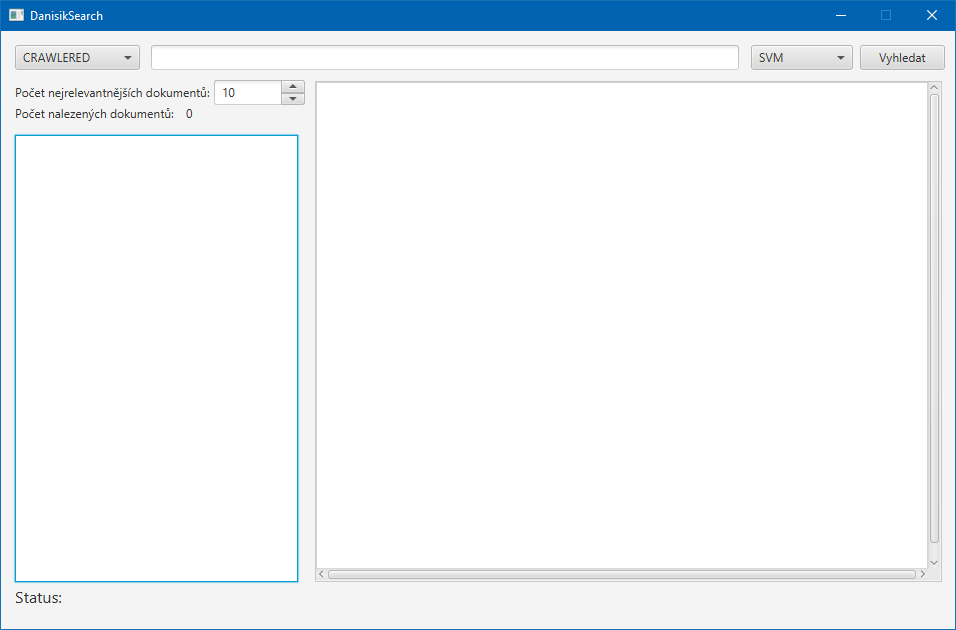
\includegraphics[width=15cm]{img/main.png}
	\caption{Hlavní okno}
	\label{fig:main}
\end{figure}

\begin{figure}[h]
	\centering
	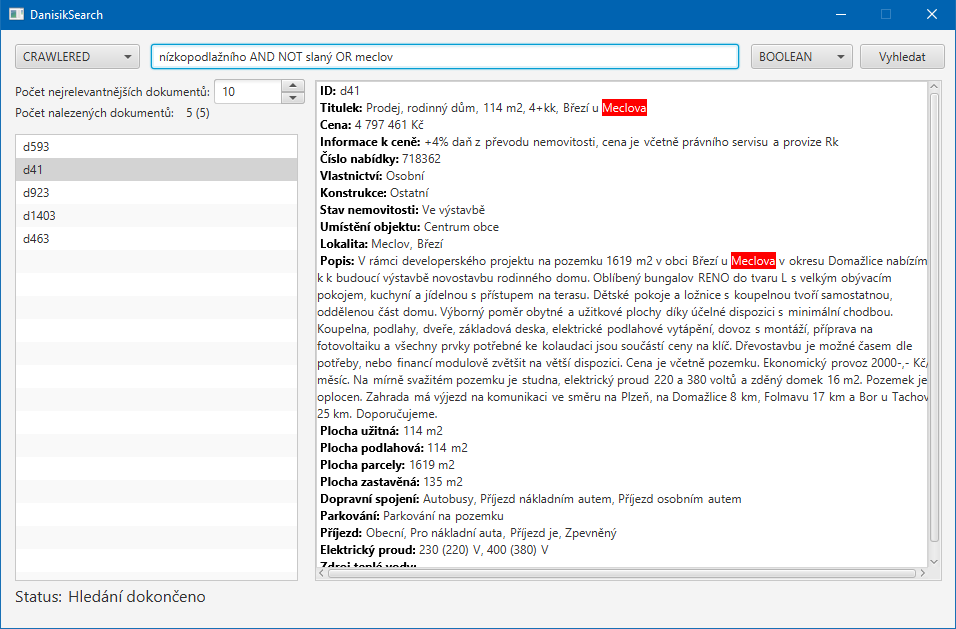
\includegraphics[width=15cm]{img/search_boolean.png}
	\caption{Boolean vyhledávání}
	\label{fig:search_boolean}
\end{figure}

\begin{figure}[h]
	\centering
	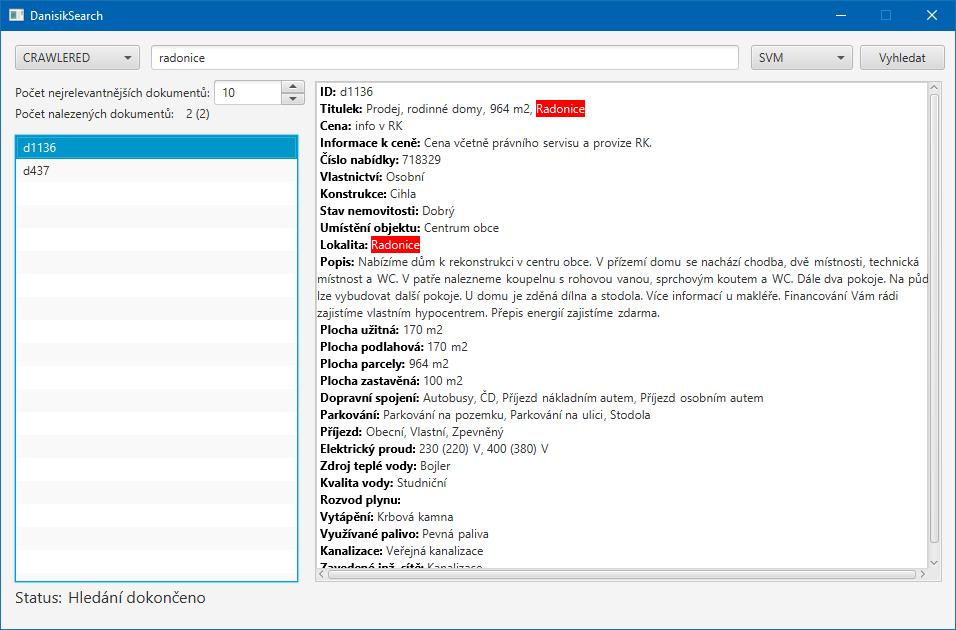
\includegraphics[width=15cm]{img/search_svm.png}
	\caption{SVM vyhledávání}
	\label{fig:search_svm}
\end{figure}

\newpage

\section{Závěr}

\begin{table}[h!]
  \begin{center}

\begin{tabular}{| c |c |}
\hline
  \textbf{Použitá pole} & \textbf{MAP}\\
\hline
Title + Description + Narrative & 0.2289\\
\hline
Title + Description & 0.1805\\
\hline
Title + Narrative & 0.2172\\
\hline
Description + Narrative & 0.2065\\
\hline
\end{tabular}
\end{center}
	\caption{MAP pro kombinace polí v query}
	\label{fig:map_combination}
\end{table}

\begin{figure}[h]
	\centering
	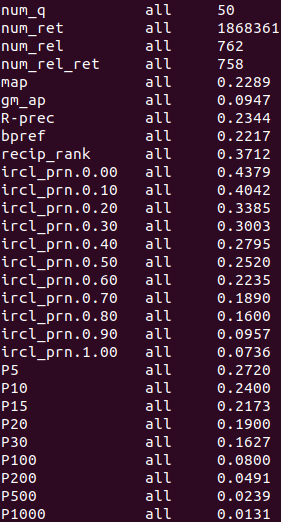
\includegraphics[width=6cm]{img/evaluation.png}
	\caption{Výsledek testu}
	\label{fig:evaluation}
\end{figure}
\end{document}